\chapter{Software operations}
\label{chap:soptware_operations}


Explain each allowed software operations (i.e. an atomic unit of treatment, a service, a functionality) including a brief description of the operation, required parameters, optional parameters, default options, required steps to trigger the operation, assumptions upon request of the operation and expected results of executing such operation.
Describe how to recognise that the operation has successfully been executed or
abnormally terminated. The template given below (i.e. section \ref{operation:MyOperation} has to be used).

Group the operations devoted to the needs of specific actors. Common
operations to several actors may be grouped and presented once to avoid redundancy.


\section{Adding task to gardeners schedule}

\hrule
\hfill
\vspace{0.5cm}
\label{operation:addTaskGardener}

The manager creates and adds a new task to be added to gardener's schedule.
\begin{description}

\item \textbf{Parameters:} nameTask, taskDescription, room, nameGardener, date,
importance
\item \textbf{Precondition:} The manager is logged in and on the manage gardener
schedule screen
\item \textbf{Post-condition:} A new task has been added to the schedule and the
new task has been assigned to the specified gardener and the manager is
notified that the task has been added.
\item \textbf{Output messages:} The \textbf{manager} will be notified that the
task has been created.

\item \textbf{Triggering:}
\begin{enumerate}
\item From within the manage gardener schedule screen, the \textbf{manger} fills
out the required entries related to the task information like the name of the task or
the date and clicks on the add button.
\item The system then adds the task now to the schedule of the gardener.
\end{enumerate}
\end{description}
\subsection{Example of adding a task}
The \textbf{manager} wants to add a watering task to the schedule, so fills out
the textinputfields as shown in the image and then he clicks on the add button.
 \begin{figure}
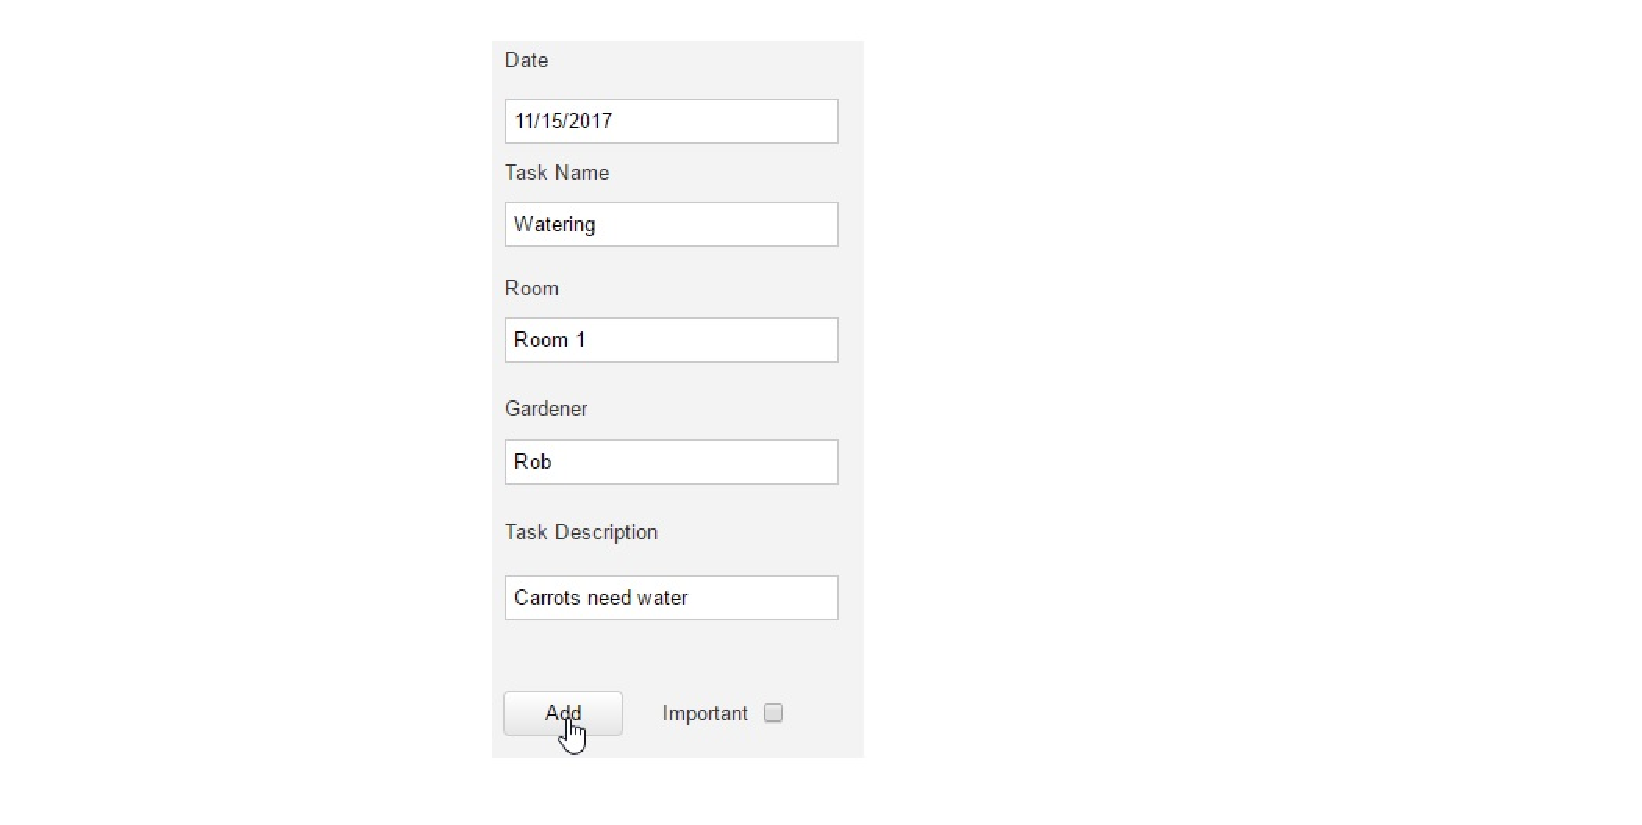
\includegraphics[width=1\textwidth]{images/addingTaskGardener.eps}
 \end{figure}


\section{Adding task to technician schedule}

\hrule
\hfill
\vspace{0.5cm}
\label{operation:addTaskTechnichian}

The manager creates and adds a new task to be added to technician's schedule.
\begin{description}

\item \textbf{Parameters:} nameTask, taskDescription, room, nameTechnician,
date, importance
\item \textbf{Precondition:} The manager is logged in and on the manage gardener
schedule screen.
\item \textbf{Post-condition:} A new task has been added to the schedule and the
new task has been assigned to the specified technician and the manager is
notified that the task has been added.
\item \textbf{Output messages:} The \textbf{manager} will be notified that the
task has been created.

\item \textbf{Triggering:}
\begin{enumerate}
\item From within the managa technician schedule screen, the \textbf{manger}
fills out the required entries related to the task information like the name of the task or
the date and clicks on the add button.
\item The \textbf{manager} The system now adds the task to the schedule of the
technician.
\end{enumerate}
\end{description}
\subsection{Example of adding a task}
The \textbf{manager} wants to the technician to change sensors, so he fills out
the requied fields and then presses the add button as shown in the image.



\section{Request a new sensor}

\hrule
\hfill
\vspace{0.5cm}
\label{operation:Request a new sensor}

The Technician can request a new sensor.
\begin{description}
\item \textbf{Parameters:} NameSensor,RoomNumber,TechnicianName,Reason
\item \textbf{Precondition:} The system is bootedup and the technician has to be
logged in and be on the technician screen.
\item \textbf{Post-condition:} Updated request sensor table.

\item \textbf{Triggering:}
\begin{enumerate}
\item \textbf{Technician} Complets the diffrent input fields and presses the
button push to the manager.
\item System sends the information to the manager by updating the request
sensor table.
\end{enumerate}
\end{description}

\subsection{Example of a request of a sensor}
\textbf{Technician} complets the input text field with their given information
that means Name of the Sensor:Temperature1 RoomNumber:1 Technician Name: Bruno
and Reason Sensor Temperature 1 gives wrong information sensor is
damaged.\textbf{System} inserts this information to the manager request sensor
table.
\hfill
\vspace{0.5cm}
\hrule

\section{Accept the request for a new sensor}

\hrule
\hfill
\vspace{0.5cm}

\label{operation:Accept the request for a new sensor}

The Manager can accept a new sensor.
\begin{description}
\item \textbf{Parameters:} /
\item \textbf{Precondition:} The system is bootedup and the Manager has to be
logged in and be on the Manager request screen and a request has to be
available.
\item \textbf{Post-condition:} Validation of the request send to the Technician.

\item \textbf{Triggering:}
\begin{enumerate}
\item \textbf{Manager} Presses the green button to validate the request.
\item System sends a message that the sensor can be added to the room to the
technican.
\end{enumerate}
\end{description}

\subsection{Example of accepting a request}
\textbf{Maneger} presses the green button to accept the request from the
Temperature1 Sensor. \textbf{System} sends a validation message to the gardener.
\hfill
\vspace{0.5cm}
\hrule

\break

\section{Add a new sensor}

\hrule
\hfill
\vspace{0.5cm}

\label{operation:Add a new sensor}
The Technician can add a sensor which has been maid available from the manager.
\begin{description}
\item \textbf{Parameters:} SensorName,Value,Room,TechnicianName,UpdateSchedule
\item \textbf{Precondition:} The system is bootedup and the Technician has to be
logged in and be on the Tehcnician screen and a request to add a sensor has to
be available.
\item \textbf{Post-condition:} The sensor has been successfully updated with the
sensor which has been added.
\item \textbf{Triggering:}
\begin{enumerate}
\item \textbf{Technician} complets the diffrent input text fields and presses
the green add button .
\item System pushes now the information to the sensor table and updates it by
adding the sensor with the other informations added.
\end{enumerate}
\end{description}

\subsection{Example of adding a new sensor}
\textbf{Technician} complets the given input text fields with the sensor name
:Temperature1 value 32 degrees and the room: 1 technician name :Bruno and the
update schedule is 15. \textbf{System} pushes the information to the sensor
table and displays the new updated table.
\hfill
\vspace{0.5cm}
\hrule



\section{Remove  requested sensor}

\hrule
\hfill
\vspace{0.5cm}
\label{operation:Request a new sensor}

The Technician can remove the requested sensor from the request table.
\begin{description}
\item \textbf{Parameters:} /
\item \textbf{Precondition:} The system is bootedup and the technician has to be
logged in and be on the technician screen and a request should be in the
request sensor table.
\item \textbf{Post-condition:} Removes the requested sensor from the sensor
request table.

\item \textbf{Triggering:}
\begin{enumerate}
\item \textbf{Technician} presses the red button on request sensor table.
\item System removes sensor from the request table.
\end{enumerate}
\end{description}

\subsection{Example of a removing of a sensor}
\textbf{Technician} presses the red button on the ligne 1 of the table where
temperature1 and which room = 1. The system removes the sensor from the request
list.

\hfill
\vspace{0.5cm}
\hrule



\break



\section{Ask for a diffrent crops}

\hrule
\hfill
\vspace{0.5cm}

\label{operation:Ask for a diffrent crop}

The gardener can request a diffrent crop which isn't already in the crops
inventory.
\begin{description}
\item \textbf{Parameters:} CropName,Amount
\item \textbf{Precondition:} The system is bootedup and the Gardener has to be
logged in and be on the Gardener screen.
\item \textbf{Post-condition:} The request has been send by adding it on the
request crop table.
\item \textbf{Triggering:}
\begin{enumerate}
\item \textbf{Gardener} complets the diffrent input text fields and presses
the ask for a non existing crop button.
\item \textbf{System} displays a pop up of the entered information.
\item \textbf{Gardener} accepts the pop up.
\item \textbf{System} pushes the information to the manager request crop table
and updates it.
\end{enumerate}
\end{description}

\subsection{Example of accepting a request}
\textbf{Technician} complets the given input text fields with the Name Mango and
amount 50. \textbf{System} displays the pop up of the information enterer Mango
and 50.\textbf{Gardener} accepts the pop up.\textbf{System} updates the request
crop table by adding Mango and amount to the table.
\hfill
\vspace{0.5cm}
\hrule



\section{Accept a diffrent crop}

\hrule
\hfill
\vspace{0.5cm}

\label{operation:Accept a diffrent crop}

The Manager can accept the request for a new crop which is not already on the
crop inventory table.
\begin{description}
\item \textbf{Parameters:}/
\item \textbf{Precondition:} The system is bootedup and the Manager has to be
logged in and be on the Manager request screen.
\item \textbf{Post-condition:} The request has been validated and the crop
inventory table has been updated by adding the requested crop.
\item \textbf{Triggering:}
\begin{enumerate}
\item \textbf{Manager} presses the green button to validated the request.
\item \textbf{System} adds the crop to he request Crop table.

\end{enumerate}
\end{description}

\subsection{Example of accepting a request}
\textbf{Manager} accepts by pressing the green button on COCO with the amount
50.\textbf{System} updates the crops invenotry table by adding the requested
crop to the crops inventory table.
\hfill
\vspace{0.5cm}
\hrule
 
\break
\section{Remove Crops from Inventory}

\hrule
\hfill
\vspace{0.5cm}

\label{operation:RemoveCrops}

The manager can remove a given kind of crops completly.
\begin{description}

\item \textbf{Parameters:} NameCrops, Amount
\item \textbf{Precondition:} The system is bootedup and manager has to be
logged in and be on the manager request screen.
\item \textbf{Post-condition:} Request table has been updated with the removed
crop.

\item \textbf{Triggering:}
\begin{enumerate}
\item \textbf{Manager} presses the red button on the crops inventory table.
\item System removes the crops from the crops inventory on the manager and
gardener screen.
\end{enumerate}
\end{description}

\subsection{Example of removing crops}
\textbf{Manager} removes the crops by pressing the red button. The System
updates the changes on the manager request screen and Gardener screen.
\hfill
\vspace{0.5cm}
\hrule


\section{Sort request crops by amount ascending order}

\hrule
\hfill
\vspace{0.5cm}

\label{operation:sortCropsRequest}

The manager can sort the crops which are requested by ascanding order.
\begin{description}

\item \textbf{Parameters:} /
\item \textbf{Precondition:} The system is bootedup and manager has to be
logged in and be on the manager request screen.
\item \textbf{Post-condition:} Request crops table has been ordered in ascanding
order.

\item \textbf{Triggering:}
\begin{enumerate}
\item \textbf{Manager} presses the top arrow.
\item System sorts the list by amount value by ascending order.
\end{enumerate}
\end{description}

\subsection{Example of removing crops}
\textbf{Manager} presses the arraw on the request crop table. System sorts the
the table by amount in ascending order.

\hfill
\vspace{0.5cm}
\hrule

\break

\section{Modify/Retrive crops Amount}

\hrule
\hfill
\vspace{0.5cm}
\label{operation:modifyCropsAmount}
The \textbf{Gardener} can modify the amount of crops on the crops inventory
table.
\begin{description}
\item \textbf{Parameters:} Name,amount
\item \textbf{Precondition:} The system is bootedup and the gardener has to be
logged in and be on the Gardener sreen.
\item \textbf{Post-condition:} Crops inventory has been modifyed on manager and
gardener screen.

\item \textbf{Triggering:}
\begin{enumerate}
\item \textbf{Gardener} Complets the input text fields and presses the modify
button.
\item System updates the table of crop inventory and adds a the time of
retriving to the manager retriving Gardener table adn reloads the screen.
\end{enumerate}
\end{description}

\subsection{Example of removing crops}
\textbf{Gardener} enters the two input fields name = Tomatoe and amount=10.
The system retrives the amount which is equal to 10 from the inventory amount of
the name Tomatoe.
\hfill
\vspace{0.5cm}
\hrule



















\section{Add crop to the inventory}

\hrule
\hfill
\vspace{0.5cm}

\label{operation:Accept a diffrent crop}

The Manager can accept the request for a new crop which is not already on the
crop inventory table.
\begin{description}
\item
\textbf{Parameters:}Name,Amount,ph-Amount,Vegtable(boolean),TemperaturePreference
\item \textbf{Precondition:} The system is bootedup and the Manager has to be
logged in and be on the Manager screen and a request has to be accepted by the
manager.
\item \textbf{Post-condition:} The invenotry has been updated by adding the
attributes to the table.
\item \textbf{Triggering:}
\begin{enumerate}
\item \textbf{Manager} complets the formula and presses the add button.
\item \textbf{System} shows a pop up of the entered values.
\item \textbf{Manager} accepts the pop up request.
\item \textbf{System} displays a message of success and adds the values to the
inventory crop table.

\end{enumerate}
\end{description}

\subsection{Example of accepting a request}
\textbf{Manager} complets the given inputs text field with the
Name: Coconut and amount 50 and ph value 9 and Vegtable false
(not coching the crop field) and temperature preference : 34. \textbf{System}
displays a pop up  what the user has entered in this case Coconut 50 9 (false)
and 34.Manager accepts the pop up by pressing the green button. System updates
the crop inventory table by adding the input values from the manager to the
table.
\hfill
\vspace{0.5cm}
\hrule






















\break

\section{Filter by sensor type}

\hrule
\hfill
\vspace{0.5cm}

\label{operation:filterSensorTable}

The \textbf{Technician} can filter the table by filter type.
\begin{description}

\item \textbf{Parameters:} /
\item \textbf{Precondition:} The system is bootedup and Technician has to be
logged in and be on the technician screen.
\item \textbf{Post-condition:} The table on the screens show only the filtered
values.

\item \textbf{Triggering:}
\begin{enumerate}
\item \textbf{Technician} choses on the top down menu a sensor type.
\item System filters out all the non equal types and doesn't display them.
\end{enumerate}
\end{description}

\subsection{Example of filtering the Sensors}
\textbf{Technician} choses a type on a the top down menu Temperature. System
know doesn't display the sensor where the type isn't equal to Temperature.
\hfill
\vspace{0.5cm}
\hrule






\section{Removes sensor from Sensor Array}

\hrule
\hfill
\vspace{0.5cm}

\label{operation:removesSensor}

The \textbf{Technician} removes the a specific sensor from the table.
\begin{description}

\item \textbf{Parameters:} /
\item \textbf{Precondition:} The system is bootedup and Technician has to be
logged in and be on the technician screen.
\item \textbf{Post-condition:} The table of sensors has been updated on the
technician and gardener screen.

\item \textbf{Triggering:}
\begin{enumerate}
\item \textbf{Technician} choses the sensor which he wants to delete and presses
the red button.
\item System removes the sensor from the table.
\end{enumerate}
\end{description}

\subsection{Example of removing Sensor}
\textbf{Technician} choses a given sensors on the Sensor table Temperature 1
sensor and presses the red button on the same line.
System removes the line from the table and reloads the screen to update it.

 \hfill
\vspace{0.5cm}
\hrule



\break
\section{Build Temperature Line Diagram}
\label{operation:BuildTemperatureDiagram}
The system draws the line diagram for the temperature of the selected room of
the dropdown menu next to it.

\begin{description}

\item \textbf{Parameters:} HistoryOfTemperaturesInAllRooms
\item \textbf{Precondition:} The system is bootedup and any actor is logged in.
\item \textbf{Post-condition:} The corresponding diagram will be drawn and
shown.

\item \textbf{Triggering:}
\begin{enumerate}
\item If at any time the \emph{statistics} page is accessed.
\end{enumerate}
\end{description}

\subsection{Example of Build Temperature Line Diagram}
The logged in user wants to see the statistics of the past days.
The user clicks on the \emph{statistics} page in the menu.
The system will now draw the temperature line diagram.




\section{Build Current Stock Bar Diagram}
\label{operation:BuildCurrentStockDiagram}
The system draws the bar diagram of the current stock of the inventory.

\begin{description}

\item \textbf{Parameters:} CurrentStockOfSeeds
\item \textbf{Precondition:} The system is bootedup and any actor is logged in.
\item \textbf{Post-condition:} The corresponding diagram will be drawn and
shown.

\item \textbf{Triggering:}
\begin{enumerate}
\item If at any time the \emph{statistics} page is accessed.
\end{enumerate}
\end{description}

\subsection{Example of Build Current Stock Bar Diagram}
The logged in user wants to see the current stock of the inventory.
The user clicks on the \emph{statistics} page in the menu.
The system will now draw the current stock bar diagram.



\break
\section{Build Water Consumption And Luminosity Level Bar And Line Diagram}
\label{operation:BuildWaterConsumptionAndLuminosityLevelDiagram}
The system draws the bar and line diagram for the water consumption in
milliliter and the luminosity level in spectral power of the selected room of
the dropdown menu next to it.

\begin{description}

\item \textbf{Parameters:} HistoryOfWaterConsumptionInAllRooms,
HistoryOfLuminosityLevelInAllRooms
\item \textbf{Precondition:} The system is bootedup and any actor is logged in.
\item \textbf{Post-condition:} The corresponding diagram will be drawn and
shown.

\item \textbf{Triggering:}
\begin{enumerate}
\item If at any time the \emph{statistics} page is accessed.
\end{enumerate}
\end{description}

\subsection{Example of Build Water Consumption And Luminosity Level Bar And Line
Diagram}
The logged in user wants to see the statistics of the past days.
The user clicks on the \emph{statistics} page in the menu.
The system will now draw the temperature line diagram.




\section{Show Crop statistics}
\label{operation:ShowCropStatistics}
The system shows the statistics of the crop \emph{(Date harvested, Plant
harvested, Number of plants harvested, Total weigth of the harvest)} and
calulates the \emph{Average weigth/plant, Days until the plants were harvested
and the growth per day}.

\begin{description}

\item \textbf{Parameters:} DatePlanted, DateHarvested, PlantHarvested,
NumberOfPlants, TotalWeigthOfCrop
\item \textbf{Precondition:} The system is bootedup and any actor is logged in.
\item \textbf{Post-condition:} The corresponding information will be calculated
and shown.

\item \textbf{Triggering:}
\begin{enumerate}
\item If at any time the \emph{statistics} page is accessed.
\item The logged in user chooses a different crop from the crop list on the
\emph{statistics} page.
\end{enumerate}
\end{description}


\subsection{Example of Show Crop statistics}
The logged in user wants to see the statistics of the past crops.
The user clicks on the \emph{statistics} page in the menu.
The system will now calculate and show the information on the latest crop.
The user wants to see older crops and triggers this system operation by choosing
a different crop.


\break
\section{Automatical Creation of Alert for Sensors}
\label{operation:AddAlertForSensors}
The system checks the incoming signal from all the different sensors for invalid
data or no incoming signal.

\begin{description}

\item \textbf{Parameters:} SensorData
\item \textbf{Precondition:} The system is bootedup.
\item \textbf{Post-condition:} AlertsDatabase is updated with a new entry.

\item \textbf{Triggering:}
\begin{enumerate}
\item The Sensors transmit invalid or impossible data.
\item The Sensors transmit no data.
\end{enumerate}
\end{description}

\subsection{Example of Automatical Creation of Alert for Sensors}
The system is bootedup and is monitoring the signal of the sensors.
Now one of the sensors sends invalid data (example: Humidity Sensor sends data
with more than 100 percent humidity) or lost the connection for whatever reason
to the system, an entry will be added into the alerts database.




\section{Automatical Creation of Alert for Warnings}
\label{operation:AddAlertForWarnigns}
The system checks the incoming signal from the humidity and temperature sensors
for data which is out of the pre-defined range.

\begin{description}

\item \textbf{Parameters:} SensorData
\item \textbf{Precondition:} The system is bootedup.
\item \textbf{Post-condition:} AlertsDatabase is updated with a new entry.

\item \textbf{Triggering:}
\begin{enumerate}
\item The Sensors transmit data out of the pre-defined range
\end{enumerate}
\end{description}

\subsection{Example of Automatical Creation of Alert for Warnings}
The system is bootedup and is monitoring the signal of the sensors.
Now the temperature sensors sends a temperature of 18 degrees celsius. The
pre-defined range for the temperature is from 20 to 27 degrees. The system will
add a warning to the alerts database, the temperature is too low.






















\break



\section{Humidty sensor push information}

\hrule
\hfill
\vspace{0.5cm}
\label{operation:Humidty sensor push information}

The Humidity Sensor pushes the information to the sensor table.
\begin{description}
\item \textbf{Parameters:} 
\item \textbf{Precondition:} The system is bootedup with the respected
configurations.
\item \textbf{Post-condition:} Updated sensor value in sensor table.

\item \textbf{Triggering:}
\begin{enumerate}
\item \textbf{Humidity sensor} send digital signal to the system.
\item System updates the value of the given sensor in the sensor table.
\end{enumerate}
\end{description}

\subsection{Example of humidity sensor sending digital signal}
\textbf{Humidity sensor 1} sends 40 as digital signal. \textbf{System} updates
the sensor table value from room 1 and humidity sensor1.
\hfill
\vspace{0.5cm}
\hrule


\section{Temperature sensor push information}

\hrule
\hfill
\vspace{0.5cm}
\label{operation:Temperature sensor push information}

The Temperature Sensor pushes the information to the sensor table.
\begin{description}
\item \textbf{Parameters:} 
\item \textbf{Precondition:} The system is bootedup with the respected
configurations.
\item \textbf{Post-condition:} Updated sensor value in sensor table.

\item \textbf{Triggering:}
\begin{enumerate}
\item \textbf{Temperature sensor} sends digital signal to the system.
\item System updates the value of the given temperature sensor in the sensor
table.
\end{enumerate}
\end{description}

\subsection{Example of humidity sensor sending digital signal}
\textbf{Temperature sensor 1} sends 24 as digital signal. \textbf{System}
updates the sensor table value from room 1 and Temperature sensor1 by modifing
the value to 24.
\hfill
\vspace{0.5cm}
\hrule

\break
\section{Light sensor push information}

\hrule
\hfill
\vspace{0.5cm}
\label{operation:Light sensor push information}

The  Light Sensor pushes the information to the sensor table.
\begin{description}
\item \textbf{Parameters:} 
\item \textbf{Precondition:} The system is bootedup with the respected
configurations.
\item \textbf{Post-condition:} Updated Light value in sensor table of the given
Light sensor.

\item \textbf{Triggering:}
\begin{enumerate}
\item \textbf{Light sensor} sends digital signal to the system.
\item System updates the value of the given sensor in the sensor table.
\end{enumerate}
\end{description}

\subsection{Example of humidity sensor sending digital signal}
\textbf{Light sensor 1} sends 550 nm as digital signal. \textbf{System}
updates the sensor table value from room 1 and updates the light value to 550nm.
\hfill
\vspace{0.5cm}
\hrule


\section{Motion sensor push information}

\hrule
\hfill
\vspace{0.5cm}
\label{operation:Motion sensor push information}

The Motion Sensor pushes the information to the sensor table.
\begin{description}
\item \textbf{Parameters:} \
\item \textbf{Precondition:} The system is bootedup with the respected
configurations.
\item \textbf{Post-condition:} The system sends alert to the manager.

\item \textbf{Triggering:}
\begin{enumerate}
\item \textbf{Motion sensor} sends digital signal to the system if any movement
is detected.
\item System displays an alert to the manager that there might be an intrusion.
\end{enumerate}
\end{description}

\subsection{Example of Motion sensor sending digital signal}
\textbf{Motion sensor 1} sends a digital signal to the system. The system alerts
the manager of an intrusion.
\hfill
\vspace{0.5cm}
\hrule

\break



\section{Turn on Heater}

\hrule
\hfill
\vspace{0.5cm}
\label{operation:Turn on heater}

In case the Temeprature sensor sends an a value less then 15 degrees the heater
is switched on.
\begin{description}
\item \textbf{Parameters:} temperatureOfSensor
\item \textbf{Precondition:} The system is bootedup with the respected
configurations and digital signals comming from the Temperature sensor which is
less then 15 degrees.
\item \textbf{Post-condition:} Heater in a given room is on until the
Temperature sensor sends value heigher than 19.

\item \textbf{Triggering:}
\begin{enumerate}
\item \textbf{Temperature sensor} sends digital signal of 14 to the system.
\item System enables the heater for the given room.
\end{enumerate}
\end{description}

\subsection{Example of humidity sensor sending digital signal}
\textbf{Temperature sensor 1} sends 14 as digital signal. \textbf{System}
enables the heater to heat the room1 until the temperature sensor sends a value
heigher than 18.
\hfill
\vspace{0.5cm}
\hrule


\section{Turn on LED}

\hrule
\hfill
\vspace{0.5cm}
\label{operation:Turn on LED}

Incase the light sensor pushes a value less than 400 the LEDs qre turned on.
\begin{description}
\item \textbf{Parameters:} lightValue,timeTicker
\item \textbf{Precondition:} The system is bootedup with the respected
configurations and digital signals comming from the Lightsensor has to be less
than 400 nm and the ticker has to be 0.
\item \textbf{Post-condition:} The LEDS for the given room are turned on until
the outside Lightsensor gives a value more than 400.

\item \textbf{Triggering:}
\begin{enumerate}
\item \textbf{Light sensor} sends digital signal of less than 400 nm to the
system.
\item System enables the LEDs for the given room if the TimeTicker is 0.
\end{enumerate}
\end{description}

\subsection{Example of humidity sensor sending digital signal}
\textbf{Light sensor 1} sends 399 as digital signal. \textbf{System}
evaluates if the timeTicker is 0 if it is it turns the LEDs on.
\hfill
\vspace{0.5cm}
\hrule




\break




\section{Open Windows}

\hrule
\hfill
\vspace{0.5cm}
\label{operation:Open Windows}

Incase the temperature sensor inside has a value higher than the value allowed.
\begin{description}
\item \textbf{Parameters:} Temperature,room,TemperatureSHouldBE
\item \textbf{Precondition:} The system is bootedup with the respected
configurations and digital signals comming from the Temperature sensor has to be
more than a given value.
\item \textbf{Post-condition:} The Windows for that given room are opend.

\item \textbf{Triggering:}
\begin{enumerate}
\item \textbf{Temperature sensor} sends digital signal of more than a given
value degrees to the system.
\item System opens the windows unitl the temperature decreeces to the requested
temperature.
\end{enumerate}
\end{description}

\subsection{Example of humidity sensor sending digital signal}
\textbf{Temperature sensor 1} sends 45 (degree) as digital signal.
\textbf{System} checks if the temperature is acceding the temperature should be
than the windows are opening.
\hfill
\vspace{0.5cm}
\hrule




\section{Turn on LED}

\hrule
\hfill
\vspace{0.5cm}
\label{operation:Turn on LED}

Incase the light sensor pushes a value less than 400 the LEDs qre turned on.
\begin{description}
\item \textbf{Parameters:} lightValue,timeTicker
\item \textbf{Precondition:} The system is bootedup with the respected
configurations and digital signals comming from the Lightsensor has to be less
than 400 nm and the ticker has to be 0.
\item \textbf{Post-condition:} The LEDS for the given room are turned on until
the outside Lightsensor gives a value more than 400.

\item \textbf{Triggering:}
\begin{enumerate}
\item \textbf{Light sensor} sends digital signal of less than 400 nm to the
system.
\item System enables the LEDs for the given room if the TimeTicker is 0.
\end{enumerate}
\end{description}

\subsection{Example of humidity sensor sending digital signal}
\textbf{Light sensor 1} sends 399 as digital signal. \textbf{System}
evaluates if the timeTicker is 0 if it is it turns the LEDs on.
\hfill
\vspace{0.5cm}
\hrule

\break


\section{Turn on watering}

\hrule
\hfill
\vspace{0.5cm}
\label{operation:Turn on watering}

Incase the humidty sensor gives a value below the requested value watering is
turned on.
\begin{description}
\item \textbf{Parameters:} humidityLevel,Room
\item \textbf{Precondition:} The system is bootedup with the respected
configurations and digital signals comming from the humidty sensor has to be
less than a given level.
\item \textbf{Post-condition:} The watering is turned on for the given room.

\item \textbf{Triggering:}
\begin{enumerate}
\item \textbf{Humidty sensor} sends digital signal of less than the accepted
amount to the system.
\item System enables the watering for a given room until the humidty level is
as the room humidtyi accepts it.
\end{enumerate}
\end{description}

\subsection{Example of Enabling wateringl}
\textbf{Humidity sensor 1} sends a value of 10 since the humidity sensor is in
room1.
\textbf{System} enables the watering for the room1 until the humidity level is
40 so that the plants have enough water.
\hfill
\vspace{0.5cm}
\hrule




